\documentclass{beamer}
\usetheme{Madrid}
\usecolortheme{default}
\usepackage{tikz}
\usepackage{algorithm}
\usepackage{algpseudocode}
\usepackage{amsmath}
\usepackage{booktabs}
\usetikzlibrary{calc, positioning, arrows.meta}
\title[LLM-LNS for MILP]{Large Language Model-driven Large Neighborhood Search for Large-Scale MILP Problems}
\author[Jongmin Mun]{Huigen Ye, Hua Xu, An Yan, Yaoyang Cheng, ICML 2025 spotlight}
\institute[]{Presenter: Jongmin Mun}
\date{USC ISE-617}

\begin{document}
	
	% Slide 1: Title
	\begin{frame}
		\titlepage
	\end{frame}
	
	% Slide 2: Motivation and Background
	\begin{frame}{Large Neighborhood Search of Mixed Integer LP}
		\begin{itemize}
			\item Scalability challenge: Branch-and-bound struggles with large MILP instances.
			\item \textbf{Large Neighborhood Search (LNS)}  starts from a feasible solution and iteratively improves solutions via Destroy and Repair operators.
			\item Bottleneck: The Destroy phase. Success depends heavily on choosing which variables to fix vs. free.	
\end{itemize}
	\end{frame}
	
	\begin{frame}{Existing strategies and limitations}
		
		\begin{itemize}
		\item Handcrafted Heuristics: Labor-intensive and task-specific. Fails to easily generalize to new problems (\emph{cold-start issue}).

\item Reinforcement Learning : Intractable search spaces. Trial-and-error exploration of RL agent is highly inefficient, leading to \emph{slow convergence}.

\item Imitation Learning  :  Requires massive amounts of high-quality labels generated by a \emph{computationally expensive}  oracle.

\item  LLM-based evolution (e.g., FunSearch, EOH):   Reliance on fixed evolutionary prompts often leads to \textbf{\emph{premature convergence}}. 
		\end{itemize}
	\end{frame}

\begin{frame}{Proposed Approach: The Dual-Layer Agent}
The core contribution is   a very smart prompt engineering
    \begin{itemize}
        \item \textbf{The Baseline:} Prior LLM methods only guide heuristic evolution  with a fixed prompt (only for combinatorial problems, not MILP)
        
        \vspace{0.2cm} % Adds a little breathing room between major points
        
        \item \textbf{The Bottleneck:} Fixed evolutionary prompts restrict exploration and cause premature convergence.
        
        \vspace{0.2cm}
        
        \item \textbf{The Solution:} A co-evolutionary, two-LLM architecture:
        \begin{itemize}
            \item \textbf{Inner Layer (Heuristic Evolution):} Given a fixed prompt, generates and refines heuristics for rapid convergence
            \item \textbf{Outer Layer (Prompt Evolution):} Improves the prompt  to  force new \textbf{exploration}
            \item \textbf{Explicit memory}: in the inner layer, the prompt explicitly states to learn from history (both from good and bad examples)
        \end{itemize}
    \end{itemize}
\end{frame}
	
	% Slide 5: Dual-Layer Agent - Inner Layer
	\begin{frame}{Dual-Layer Agent: Inner Layer (Heuristic Evolution)}
		The \textbf{Inner Layer} focuses on evolving heuristic strategies (thoughts and code) to ensure rapid convergence[cite: 2054, 2162].
		
		\begin{itemize}
			\item Prior LLM approaches established that language models can guide heuristic evolution.
			\item The Limitation: Fixed evolutionary prompts limit exploration.
			\item This Paper's Approach: Use two LLMs. One evolves the heuristics. The other  evolves that LLM.

					\end{itemize}
	\end{frame}
	
 

		\begin{frame}{Inner Exploitation Loop:  Evolution of Heuristics}
			\vskip -2mm
		 Exploitation: find the best possible heuristics with  evolution prompt fixed
		 \vskip 3mm
			\centering
			% Resize the diagram to exactly the width of the slide text area
			% The '!' tells LaTeX to keep the aspect ratio the same
			\resizebox{\textwidth}{!}{%
				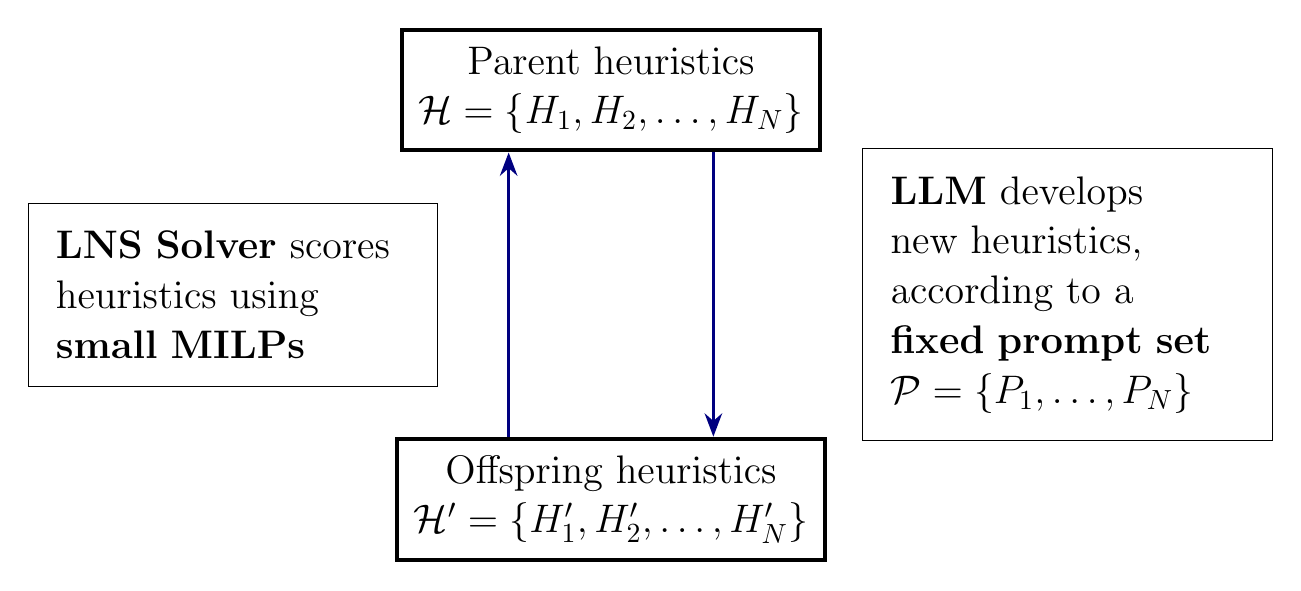
\begin{tikzpicture}[
					centerbox/.style={
						draw,
						rectangle,
						align=center,
						inner sep=6pt,
						line width=1.5pt,
						font=\Large
					},
					sidebox/.style={
						draw,
						rectangle,
						align=left,
						inner sep=10pt,
						text width=4.5cm,
						font=\Large
					}
					]
					
					% Main boxes
					\node (parent) [centerbox] at (0, 2.6) {Parent heuristics \\ $\mathcal{H}  = \{ H_1, H_2, \ldots, H_N \}$};
					\node (offspring) [centerbox] at (0, -2.6) {Offspring heuristics \\ $\mathcal{H}' = \{ H_1', H_2', \ldots, H_N' \}$};
					
					% Left/Right boxes 
					\node (solver) [sidebox] at (-4.8, 0) {\textbf{LNS Solver} scores heuristics using \textbf{small MILPs}};
					\node (llm) [sidebox] at (5.8, 0) {\textbf{LLM} develops new heuristics, according to a \textbf{fixed prompt set} $\mathcal{P} = \{P_1, \ldots, P_N\}$};
					
					% Arrows 
					\draw [-{Stealth}, line width=1.2pt, color=blue!50!black] 
					($(offspring.north)-(1.3cm, 0)$) -- ($(parent.south)-(1.3cm, 0)$);
					\draw [-{Stealth}, line width=1.2pt, color=blue!50!black] 
					($(parent.south)+(1.3cm, 0)$) -- ($(offspring.north)+(1.3cm, 0)$);
					
				\end{tikzpicture}%
			} 
	Repeat   for a fixed number of time; the whole procedure can be written as 
\begin{equation*}
	\mathcal{H}= \texttt{inner}(\texttt{prompt})
\end{equation*}		
			% End of resizebox
		\end{frame}
		

\begin{frame}
	\begin{itemize}
		\item Generation 0: capacity ratio with penalties
		\begin{equation*}
			\text{scores}[\text{bins} > \text{item}] = \frac{\text{bins} - \text{item}}{\text{bins}} \times \frac{1}{\text{index of bin} + 0.5} 
		\end{equation*}
		
		\item Generation 5:  Random exploration factor added
		\begin{align*}
			\text{scores}[\text{bins} > \text{item}] &= \frac{\text{bins} - \text{item}}{\text{bins} + 10^{-5}} - \frac{
				\frac{\text{bins}^2}{10^2}
			}{
				\max\left(\frac{\text{bins}^2}{10^2}\right)
			} \left( 1 - \frac{\text{bins} - \text{item}}{\max(\text{bins})} \right) 
			\\& \quad + \text{randomness} \times 0.1 
		\end{align*}
		
		\item Generation 8: Advanced hybrid optimization methods, such as genetic algorithms combined with tabu search, are introduced
		\begin{align*}
			\text{scores}[\text{bins} > \text{item}] &= \frac{\text{bins} - \text{item}}{\text{bins} + 10^{-5}} - \text{history penalty} - \frac{
				\frac{\text{bins}^2}{15^2}
			}{\max\left(\frac{\text{bins}^2}{15^2}\right)} 
			\\& \quad + \text{mutation variance} - \left( 1 - \frac{\text{bins} - \text{item}}{\max(\text{bins}) + 10^{-5}} \right) 
		\end{align*}
	\end{itemize}
\end{frame}
\begin{frame}{Outer Exploration Loop: Evolution of Prompts}
	\vskip -2mm
	Exploration: when inner loop stagnates, change the prompt
	\vskip 3mm
	\centering
	
	% Added [H] here to prevent Beamer floating errors
	\begin{algorithm}[H]
		\caption{Outer loop for exploration}
		\begin{algorithmic}[1] % [1] enables line numbering
			\Require Initial heuristic $H_0$, Initial prompt $P$, Total iterations $T$
			\For{$t = 1$ \textbf{to} $T$}
			\State $\mathcal{H}_{t} \gets \text{inner}(P)$
			\If{no improvement of $\mathcal{H}_{t}$ for a certain number of steps}
			\State $P \gets \texttt{LLMevolve}(P)$
			\EndIf
			\EndFor
		\end{algorithmic}
	\end{algorithm}
	
Final step: use the best strategy out of $\mathcal{H}_T$ and run LNS on massive MILP.	
\end{frame}

\begin{frame}
	\begin{itemize}
		\item \textbf{Generation 1: Initialization by handcrafted prompts}   ``Create a completely new algorithm'', ``Modify the given algorithm'' 
		
		\item \textbf{Generation 6: Addressing Stagnation.} ``Reconfigure heuristic principles to \textbf{reduce computational complexity} while maintaining effectiveness.'' 

		
		\item \textbf{Generation 10: Stochastic Adjustment.}  ``Enhance diversity by \textbf{introducing stochastic elements} to refine exploration strategies.'' 

 
	\end{itemize}
\end{frame}
	% Slide 7: Differential Memory
\begin{frame}{Inside the LLM: Differential Memory for Directional Evolution}
	\begin{itemize}
		\item \textbf{Historical Context:} Inside the inner loop, LLM reads a set of $m$ strategy-thought-fitness tuples, capturing both successful and unsuccessful heuristics:
		$$S^{(t)} = \left\{ \langle H_i^{(t)}, \text{thought}_i, f(H_i^{(t)}) \rangle \right\}_{i=1}^m$$
		
		\item \textbf{Directional Evolution:} The \texttt{LLM} generates the next iteration by conditioning on this historical memory:
		$$H_i^{(t+1)} = \texttt{LLM}( \texttt{prompt} \parallel S^{(t)})$$
		
		\item \textbf{The  \texttt{prompt}} combines two key components:
		\begin{itemize}
			\item[--] The strategic prompt provided by the Outer Loop.
			\item[--] A differential memory instruction: \textit{``Learn from history, both good and bad. Think of what makes the difference.''}
		\end{itemize}
	\end{itemize}
\end{frame}
	
	\section{Expreiments}
	
	% Slide 9: Experimental Setup
	\begin{frame}{Experimental Setup: Task 1}
		\textbf{Task 1: Combinatorial Optimization}  		\begin{itemize}
			\item Problems: Online Bin Packing, Traveling Salesman Problem (TSP) 
			\item Baselines: 
\begin{itemize}
\item Hand-crafted heuristics
\item Neural Networks (POMO, LEHD)
\item LLM-based approaches (FunSearch, EOH)
\end{itemize}
		\end{itemize}
		
	                                	\end{frame}


% Slide 10: Results - Combinatorial Optimization
\begin{frame}{Results: Combinatorial Optimization (bin packing)}
500 bins instances:                                                                       	
	\begin{table}[h]
		\centering
		% \resizebox{\textwidth}{!}{ % Uncomment this and the closing brace below if the table is too wide
		\begin{tabular}{l ccc c}
			\toprule
			\textbf{Method / items} & \textbf{1k} & \textbf{5k} & \textbf{10k} & \textbf{Avg} \\
			\midrule
			First Fit & 4.97\% & 4.27\% & 4.28\% & 4.61\% \\
			Best Fit  & 4.50\% & 3.91\% & 3.95\% & 4.23\% \\
			FunSearch & 6.75\% & 1.47\% & 0.74\% & 2.31\% \\
			EOH       & 4.32\% & 1.06\% & 0.97\% & 2.09\% \\
			\emph{LLM-LNS}      & \textbf{3.67\%} & \textbf{0.82\%} & \textbf{0.42\%} & \textbf{1.63\%} \\
			\bottomrule
		\end{tabular}
		% } % Closing brace for \resizebox
		\label{tab:performance_c500}
	\end{table}
	
	\begin{itemize}
		\item LLM-LNS outperforms handcrafted heuristics in all instances.
		\item LLM-LNS outperforms existing LLM approaches in large instances.
		\item Not on the table, but also beats ML based methods oh large instances
	\end{itemize}
	
\end{frame}

	\begin{frame}{Experimental Setup: Task 2}
 
		
	\textbf{Task 2: Large-Scale MILP Benchmark}  		\begin{itemize}
			\item Datasets: Set Covering (SC), Minimum Vertex Cover (MVC), Maximum Independent Set (MIS), Mixed Integer Knapsack Set (MIKS) 
		 
			\item Baselines: ACP, CL-LNS, Gurobi, SCIP, GNN\&GBDT, Light-MILPOPT.
			\item No LLM-based baselines.
\end{itemize} 
                                	\end{frame}	
	% Slide 11: Results - Large-Scale MILP
	\begin{frame}{Results: Large-Scale MILP Generalization}
\begin{table}[h]
    \centering
    \begin{tabular}{l cccc}
        \toprule
        & \multicolumn{2}{c}{\textbf{MIS}} & \multicolumn{2}{c}{\textbf{MIKS}} \\
        \cmidrule(lr){2-3} \cmidrule(lr){4-5}
        \textbf{Method} & \textbf{MIS1} & \textbf{MIS2} & \textbf{MIKS1} & \textbf{MIKS2} \\
        & (Max) & (Max) & (Max) & (Max) \\
        \midrule
        Random-LNS    & 22892.9 & 223748.6 & 36011.0 & 351964.2 \\
        ACP           & 23058.0 & 226498.2 & 34190.8 & 332235.6 \\
        CL-LNS        & 15000.0 & -        & -       & -        \\
        Gurobi        & 21789.0 & 216591.3 & 32960.0 & 329642.4 \\
        SCIP          & 18649.9 & 9104.3   & 29974.7 & 168289.9 \\
        GNN\&GBDT     & 22795.7 & 227006.4 & * & * \\
        Light-MILPOPT & 22966.5 & 230432.9 & 36125.5 & 362265.1 \\
        LLM-LNS  & \textbf{23169.3} & \textbf{231636.9} & \textbf{36479.8} & \textbf{363749.5} \\
        \bottomrule
    \end{tabular}
    \caption{Performance comparison on MIS and MIKS benchmarks. Best results are highlighted in bold.}
    \label{tab:milp_benchmark_results_subset}
\end{table}
		
	
	\end{frame}
\begin{frame}{MILP efficiency}
Measured by primal integral, LLM-LNS is at least 20\% more efficient than the closest competitors
		
\end{frame}
	
	% Slide 12: Conclusion
\begin{frame}{Conclusion}
	\begin{itemize}
		\item \textbf{The Gap:} While LLM-based heuristics overcome the data and convergence limits of Imitation Learning and RL, fixed prompts often trap them in \textbf{local optima}.
		
		\vspace{0.2cm}
		
		\item \textbf{The Contribution:} A \textbf{Dual-Layer Agent} architecture.
		\begin{itemize}
			\item \textit{Outer Loop:} Dynamically evolves prompts to force exploration.
			\item \textit{Inner Loop:} Evolves heuristics by explicitly learning from both successful and failed historical attempts.
		\end{itemize}
		
		\vspace{0.2cm}
		
		\item   Empirically outperforms existing state-of-the-art methods on large-scale problems in both \textbf{objective quality} and \textbf{efficiency}, while remaining \textbf{easy to implement}.
		
	\end{itemize}
\end{frame}
\begin{frame}{Limitations}
	\begin{itemize}
		\item Heuristics are learned from and evaluated on small-sized problems. Cannot explain why it generalizes to big problems.
		\item Computationally efficient, but ignores high-quality labeled data.
	\end{itemize}
\end{frame}
	
\end{document}